\chapter{Analytical solutions of the Landau-Lifshitz-Gilbert equation}

When testing numerical methods for differential equations it is very helpful to be able to compare the results with known analytical solutions.
This section contains some solutions useful for this purpose.

\section{Solution due to Mallinson}

In a 2000 paper\cite{Mallinson2000} Mallinson gives an analytical equation for the time taken for magnetisation to ``switch'' from one polar angle (angle to the field axis) to another.
He also gives the azimuthal angle (the angle around the field axis) rotated through during this switching.

The conditions for this model to apply are:
\begin{enumerate}
\item Constant applied field.
\item No exchange field.
\item Uniaxial anisotropy.
\item Magnetostatic field (prolate ellipsoidal particles only).
\item All effective fields must lie along the same axis.
\end{enumerate}

Let $\theta_1$, $\theta_2$ be the initial and final angles between the field axis and the magnetisation (\ie initial and final polar angles in the spherical polar coordinate system with the field axis as the main axis). Let $H_k$ be the combined anisotropy field: $H_k = \frac{2 K}{M_s} + M_s(N_\perp - N_\parallel)$ where $N$ is the demagnetisation tensor of the ellipsoid. All other symbols have their usual meanings. Then the time taken to switch from $\theta_1$ to $\theta_2$ is

\begin{equation}
  \tau = \frac{\dampc^2 +1}{\gymagc \dampc} \frac{1}{H^2 - H_k^2}
  \bigb{ H \ln \bigs{ \frac{\tan(\theta_2/2)}{\tan(\theta_1/2)} }
       + H_k \ln \bigs{ \frac{H - H_k \cos\theta_1}{H - H_k \cos\theta_2} }
       + H_k \ln \bigs{ \frac{\sin\theta_2}{\sin\theta_1} }
     }.
\end{equation}

The azimuthal angle precessed through during this switching is
\begin{equation}
  \phi = \frac{-1}{\dampc} \ln \bigs{ \frac{\tan(\theta_2/2)}{\tan(\theta_1/2)} }.
\end{equation}

Note that this is not really a true ``solution'' to the Landau-Lifshitz-Gilbert equation.
It gives the switching time and azimuthal angle as a function of polar angle rather than the magnetisation direction as a function of time. However comparing the exact values with those generated by a model is still a useful test.


\section{Wave-like solution in an infinite domain}
\label{sec:wave-like-solution}

These solutions are taken from \cite{Jeong2014}, \cite{Fuwa2006}. It was originally published (as far as I can tell) in \cite{Lakshmanan1976} but in a much harder to understand form.
For most parameters the solution is just a wave-like excitation in $m_x(\xv, t)$ and $m_y(\xv, t)$ whose oscillations are damped towards a uniform $m_z = \pm 1$ state over time.
As far as I know it is the only exact solution of the LLG with non-trivial $\xv$ dependence.

For an infinite magnetic domain (\ie periodic boundary conditions) of dimension $D$ choose some constant $c \in \real$ and $\kvec \in \real^D$.
Write
\begin{equation}
  \begin{aligned}
    \that(t) &= \frac{t}{1 + \dampc^2}, \\
    b(t) &= \abs{\kvec}^2 \dampc \that(t), \\
    d(t) &= \sqrt{\sin^2(c) + \cos^2(c)e^{2 b(t)}}, \\
    g(t) &= \frac{1}{\dampc} \log \bigs{ \frac{d(t) + \cos(c) e^{b(t)}}{1 + \cos(c)} }.
  \end{aligned}
\end{equation}
Then
\begin{equation}
  \begin{aligned}
    m_x(t) &= \frac{1}{d(t)} \sin(c) \cos\bigb{\kvec \cdot \xv + g(t) }, \\
    m_y(t) &= \frac{1}{d(t)} \sin(c) \sin\bigb{\kvec \cdot \xv + g(t) }, \\
    m_z(t) &= \frac{1}{d(t)} \cos(c) e^{b(t)},
  \end{aligned}
\end{equation}
is a solution of the Landau-Lifshitz-Gilbert equation with $\heff = \lap \mv$.

The rescaling of time given by $\that(t)$ is needed to convert from a solution of the Landau-Lifshitz equation \eqref{eq:ll-nd-simpler} to a solution of the Landau-Lifshitz form of the Landau-Lifshitz-Gilbert equation \eqref{eq:ll-nd-llglike}, \ie to account for the correction to the form of the damping as introduced by Gilbert.

The function $d(t)$ is a normalisation parameter to keep $\abs{\mv(\xv, t)} = 1$ everywhere.
To see this note that $\sin^2(c) \cos^2\bigb{f(\xv)} + \sin^2(c) \sin^2\bigb{f(\xv)} = \sin^2(c)$, so the length contribution of the $x$ and $y$ terms is $\sin^2(c)$.

The vector $\kvec$ is the wave vector, it determines the direction and speed of propagation of the wave.

The parameter $c$ represents in some way the fraction of the initial magnetisation which takes part in the oscillations.
If $c = 0$ then $m_x, m_y = 0$ and there is no wave. 

\begin{figure}
  \centering
  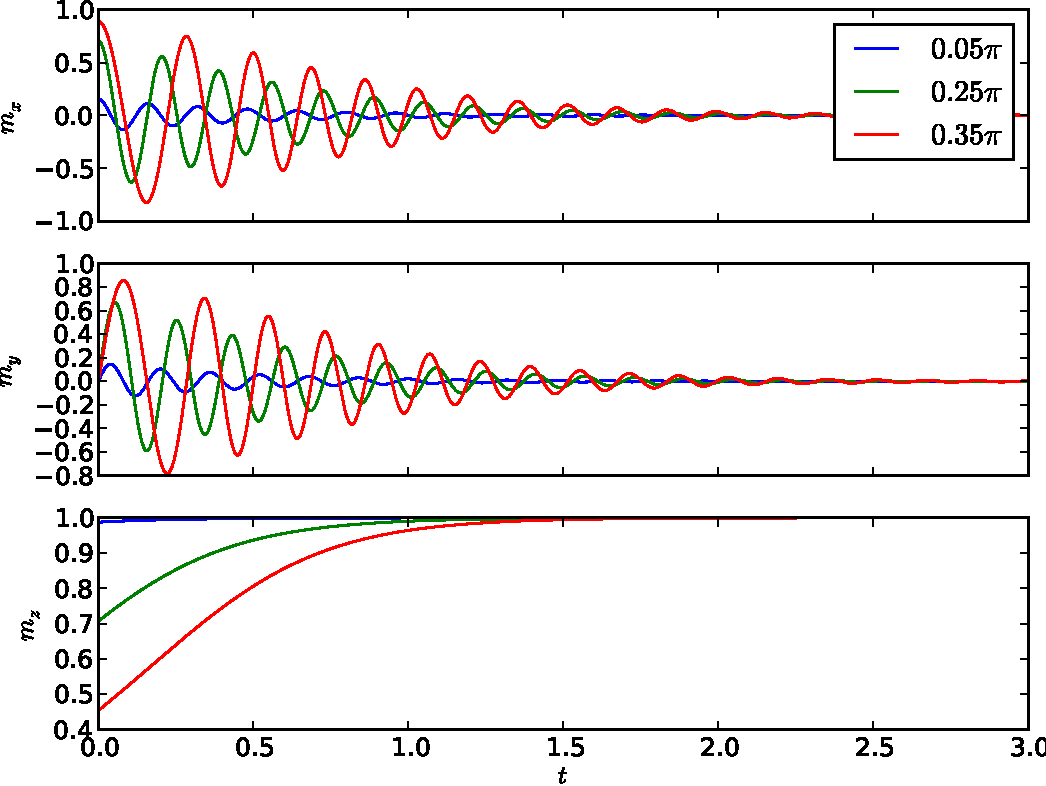
\includegraphics[width=0.8\textwidth]{plots/wave_exact_solution_parameters/exact_solution_parameters.pdf}
  \caption{One dimensional wave solution values over time at $x=0$ with $k = 2\pi$, $\dampc = 0.05$ and various $c$ well away from $\frac{\pi}{2}$.}
  \label{fig:wave-solution-vary-c}
\end{figure}

\autoref{fig:wave-solution-vary-c} shows the effect of increasing $c$ on the evolution of the magnetisation at $\xv = 0$ in one dimension and with $k = 2\pi$ and $\dampc = 0.05$.
As $c$ the initial value of $m_z$ decreases and the amplitude of the oscillations in $m_x$ and $m_y$ increase.

As $c$ approaches $\frac{\pi}{2}$ the behaviour becomes more complex, this is shown in \autoref{fig:wave-solution-vary-c-complex}.
Essentially there is an additional initial exponential decay towards a state with moderate $m_z$, after which the dynamics are similar to the lower-$c$ case.
At $c=\frac{\pi}{2}$ then $\mv(\xv, t)= (\cos(\kv\cdot\xv), \sin(\kv\cdot\xv), 0)$ and there are no dynamics.
Above $c=\frac{\pi}{2}$ the initial $m_z$ goes negative and the behaviour is symmetrical with that below $c=\frac{\pi}{2}$

\begin{figure}
  \centering
  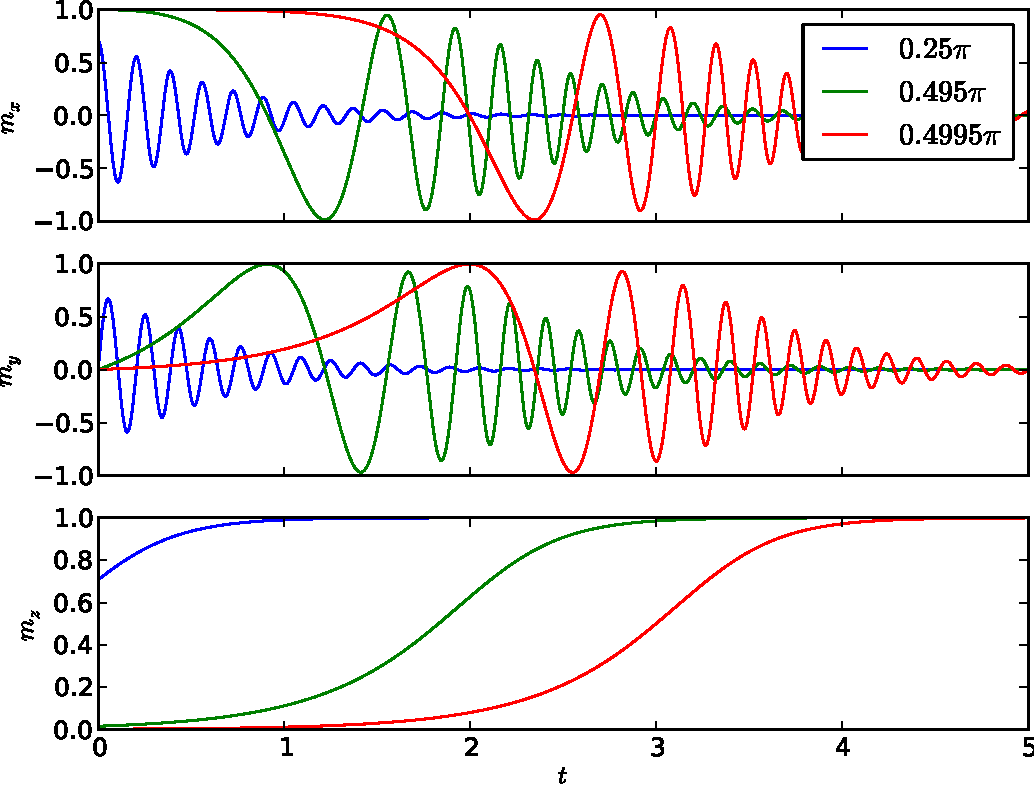
\includegraphics[width=0.8\textwidth]{plots/wave_exact_solution_parameters/exact_solution_parameters_complex.pdf}
  \caption{One dimensional wave solution values over time at $x=0$ with $k = 2\pi$, $\dampc = 0.05$ and $c$ approaching the critical value $\frac{\pi}{2}$.}
  \label{fig:wave-solution-vary-c-complex}
\end{figure}


In the limit of $\dampc \goesto 0+$ the solution becomes\cite{Fuwa2006}:
\begin{equation}
  \begin{aligned}
    m_x &= \sin(c) \cos\bigb{\kvec \cdot \xv + \abs{\kvec}^2 \cos(a) t}, \\
    m_y &= \sin(c) \sin\bigb{\kvec \cdot \xv + \abs{\kvec}^2 \cos(a) t}, \\
    m_z &= \cos(c).
  \end{aligned}
\end{equation}
This is just a simple wave in space and time.



\section{Solution due to Serpico et. al.}

Serpico et. al. \cite{Serpico2003} give a complete solution for the \emph{undamped} spatially constant Landau-Lifshitz equation.




\section{Constant field solution}

Another analytical solution based on the non-Gilbert form of the Landau-Lifshitz-Gilbert equation is given by Jiang et. al.\cite{Jiang2001}

\begin{align*}
  \phi(t) &= \gamma' H t, \\
  \cos \theta(t) &= \tanh (\gamma' \dampc H (t - t_0)), \\
  \sin \theta(t) &= \bigb{ \cosh (\gamma' \dampc H (t - t_0)) }^{-1}, \\
\end{align*}
where $\gamma' = \frac{\gymagc}{1 + \alpha^2}$ and
\begin{equation}
  t_0 = \frac{1}{\gamma' \dampc H} \log \bigs{ \frac{\sin \theta_0}{1 + \cos \theta_0} }
\end{equation}


??ds note on use as a semi-analytical time integrator


%%% Local Variables:
%%% mode: latex
%%% TeX-master: "main"
%%% End:
